\section{System overview}
The system is designed to have a primary page respesonsible for interactive elements for device selection, room detection, and data collection management. This page interacts with various services including the \texttt{BLEScannerService}, \texttt{RssiDataCollector}, \texttt{RssiDataHandler}, and \texttt{BLEAdvertisementScanner}, to carry out device scanning, data collection, and processing.
These services are connected in an event driven manner, which can be partitioned into several stages, where services are activated based on the input from the user interface. 
Figure \ref{fig:StateDiagram} is a state diagram illustrating the transitions happening from the start of the application, through the idle stage and the listening stage. 

\begin{figure}[H]
    \centering
    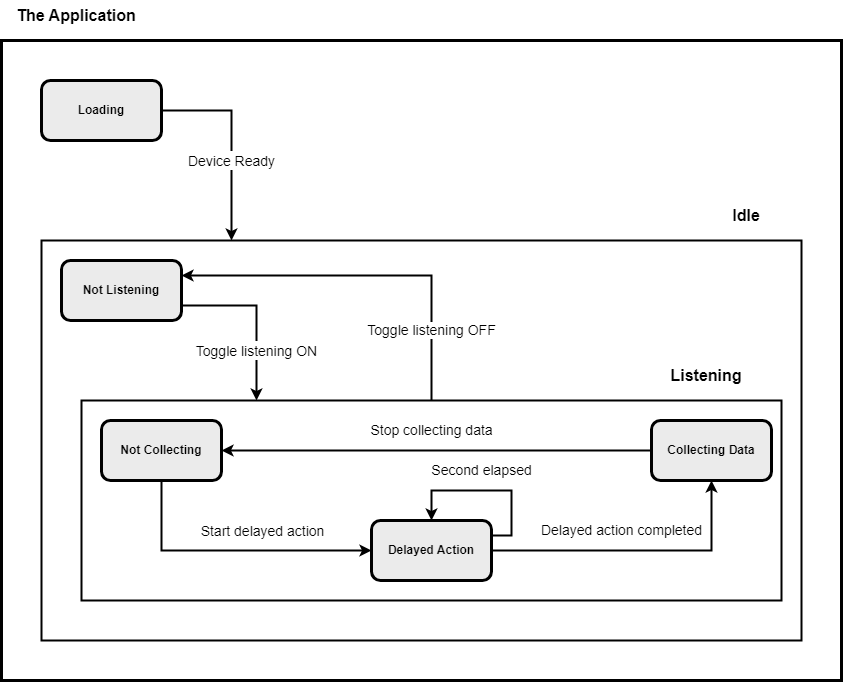
\includegraphics[width=0.8\textwidth]{images/BLE State diagram.drawio.png}
    \caption{A state diagram illustrating the event propagation}
    \label{fig:StateDiagram}
\end{figure}

These two stages, along with the states within each stage can be seen in figure \ref{fig:StateDiagram}. 
An idle mode and a listening mode. 
When the application is started, it will run background jobs that gives the device the ability to scan for other devices, collect Bluetooth beacon advertisement and RSSI data updates. 
This corresponds to the \textit{loading state}.
Once the device is ready, it will transition to a \textit{Not listening} state. 
In this state the user has the option to toggle listening on and off. 
If the user toggles listening on, the application will transition to a \textit{not collecting} state.
At this state, the device will start listening for advertisement and RSSI data updates, allowing the user to start collecting this data.
When the user starts collecting data, a delayed action will be started and the application will transition to a \textit{Delayed Action} state.
The point of this delayed action, is to allow the user to orient themselves before the data collection process starts.
Once the delayed action has finished, the application will transition to a data collecting state, which can be ended and the application will go back to a non-collecting state.

The int

